\documentclass[12]{article}
\usepackage[utf8]{inputenc}
\usepackage{cite}
\usepackage{float}
\usepackage{graphicx}
\usepackage{amssymb}
\author{Xavier Martín Ballesteros and Adrià Cabeza Sant'Anna \\ \small UNIVERSITAT POLITÈCNICA DE CATALUNYA}
\title{Flower detection using features\\ \large{Computer Vision, UPC}}


\begin{document}

%\maketitle

\begin{titlepage}
	\centering
%	{\scshape\LARGE UNIVERSITAT POLITÈCNICA DE CATALUNYA \par}
	\vspace{1cm}
	{\scshape\Large UNIVERSITAT POLITÈCNICA DE CATALUNYA\par}
	\vspace{1.5cm}
	{\huge\bfseries Computer Vision \par}
	\vspace{2cm}
	{\Large \textbf{Flower detection using features}\par}
	\vspace{0.2cm}
	{\Large Adrià Cabeza Sant'Anna and Xavier Martin Ballesteros\break \par}
	
	\vspace*{\fill}
	
\includegraphics[scale=0.4]{UPClogo.png}\par\vspace{1cm}

% Bottom of the page
	{\large \today}
\end{titlepage}

\newpage
\tableofcontents
\newpage aquí si volem 

\section{Introduction}
The aim of this assignment is to classify 12 different types of flowers using feature extraction. 

We have first implemented several ways to extract features that we believed could be key in order to classify correctly the flowers, we tested them, and using different classifiers (decisions trees, SVM or random forest) have tested the accuracy, specificity or sensitivity. 

\section{Descriptors}
In the following sections we will introduce different descriptors we have used to find those valuable features.

\subsection{Compactness}
\subsection{Color}
\subsection{Number of petals}
\begin{figure}[H]
\centering
  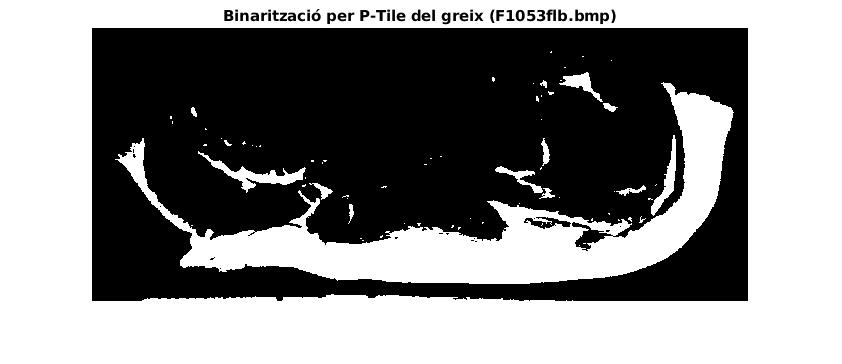
\includegraphics[scale=0.45]{output/PtileF1053flb.jpg}
  \caption{Ptile}
  \label{fig:Ptile}
    \vspace{-0.3cm}
\end{figure}


\subsection{Relative distance of the centroid}
\subsection{Hoggs form: Orientation}
\subsection{Fourier descriptor: Shape}


\section{Data augmentation}
In order \textbf{to strenghten our descriptors} we have also used the following public repository:\textit{Albumentation: fast image augmentation library and easy to use wrapper around other libraries}(see AFEGIR NUM in References for more}, which proporcionates facilities to augment the dataset including several transformations like: flipping, blurrring, RGB Shifting, Random contrast, Random brightness, etc...
\medskip

To decide which transformations we wanted to apply, we looked first to our descriptors and the importance of each feature. For example, we discarted the Channel Shuffle because we believe that the color is very important for our implementation. Then, based on trial and error, we picked some of them which gave us an overall better result. Finally we are using:
\begin{itemize}
    \item polla
    \item polla
    \item polla
\end{itemize}


\newpage
\begin{thebibliography}{100}

\bibitem{Albumentations}
    A. Buslaev (2018). Based on \textit{Albumentations: fast and flexible image augmentations} [online]. Paper available at:https://arxiv.org/abs/1809.06839. Code available at:https://github.com/albu/albumentations  [Accessed 3 June. 2019].

%%%%%%%%%%%%%%%%%%%%%%%%%%%%%%%%%%%%%%%%%%%%%%%%%%%%%%%%%%%%%%%%%%%%%%%%%%%%%%%%%%%%%%%
\bibitem{Analysis of image Thresholding Methods for application to augmented reality enviornments}
D. Martín Carabias (2012). \textit{Analysis of image Thresholding Methods for application to augmented reality enviornments.} [online] UCM. Available at: https://eprints.ucm.es/16932/1/Tesis\_Master\_Daniel\_Martin\_Carabias.pdf [Accessed 14 Mar. 2019].


\bibitem{A survey of Thresholding Techniques}
P. K. Sahoo, S. Soltani, K.C. Wong and Y.C. Chen (1988). \textit{A survey of Thresholding Techniques}. University of Waterloo, Waterloo, Canada  [Accessed 16 Mar. 2019].

\bibitem{}N. Otsu, \textit{A Threshold Selection Method from Gray-Level Histograms}, in IEEE Transactions on Systems, Man, and Cybernetics, vol. 9, no. 1, pp. 62-66, Jan. 1979.
[online] Available at http://ieeexplore.ieee.org/stamp/stamp.jsp?tp=\&arnumber=4310076\&is
number=4310064 [Acessed 17 Mar. 2019].

\bibitem{}Dr. Andrew Greensted (2010), \textit{Otsu Thresholding}. [online]. Available at http://www.labbookpages.co.uk/software/imgProc/otsuThreshold.html [Accessed 17 Mar. 2019].

\bibitem{}Senthilkumaran,  N.  \&  Sivapriya,  M.  (2017),  \textit{Riddler's  Thresholding Algorithm  for  DNA  Image  Using  ISODATA  Modified  Algorithm} Journal  of Information Technology, Vol.3, No.2, pp.41-48. [online] Available at: http://www.ijitjournal.org/volume-3/issue-2/IJIT-V3I2P9.pdf [Accessed 17 Mar. 2019].

\end{thebibliography}

\end{document}
